\subsection{Experimentación ImagenFantasma de a 4 pixeles}
\subsubsection{Hipótesis}
¿Operar con más datos mejora el rendimiento de un programa? Depende, si realiza la misma cantidad de instrucciones no se esperaría que cambie.
En nuestro caso, ¿Y si la cantidad de instrucciones ejecutadas por pixel en cada ciclo es menor? ¿O hay más instrucciones por ciclo, pero hay menos accesos a memoria?
El planteamiento de este experimento es tratar de responder ambas preguntas.

Como expliqué en el desarrollo del filtro ImagenFantasma y como muestra la figura~\ref{calcb}, si dividimos la imagen a procesar en submatrices de 2x2, el cálculo de b tiene datos en común para toda la submatriz, estos son los pixeles presentes en la submatriz correspondiente a los offset.
Entonces en lugar de procesar de a dos pixeles, y recorrer cada fila de la submatriz de los offsets dos veces  por ciclo, es decir dos veces cada pixel.
Esta implementación recorre la imagen como una matriz de submatrices de 2x2 y ya no recorre las filas de la submatriz más de una vez.
Planteado el caso, se espera que la perfomance del filtro mejore.

\subsubsection{Resultados}
\begin{figure}[h]
    \begin{center}
	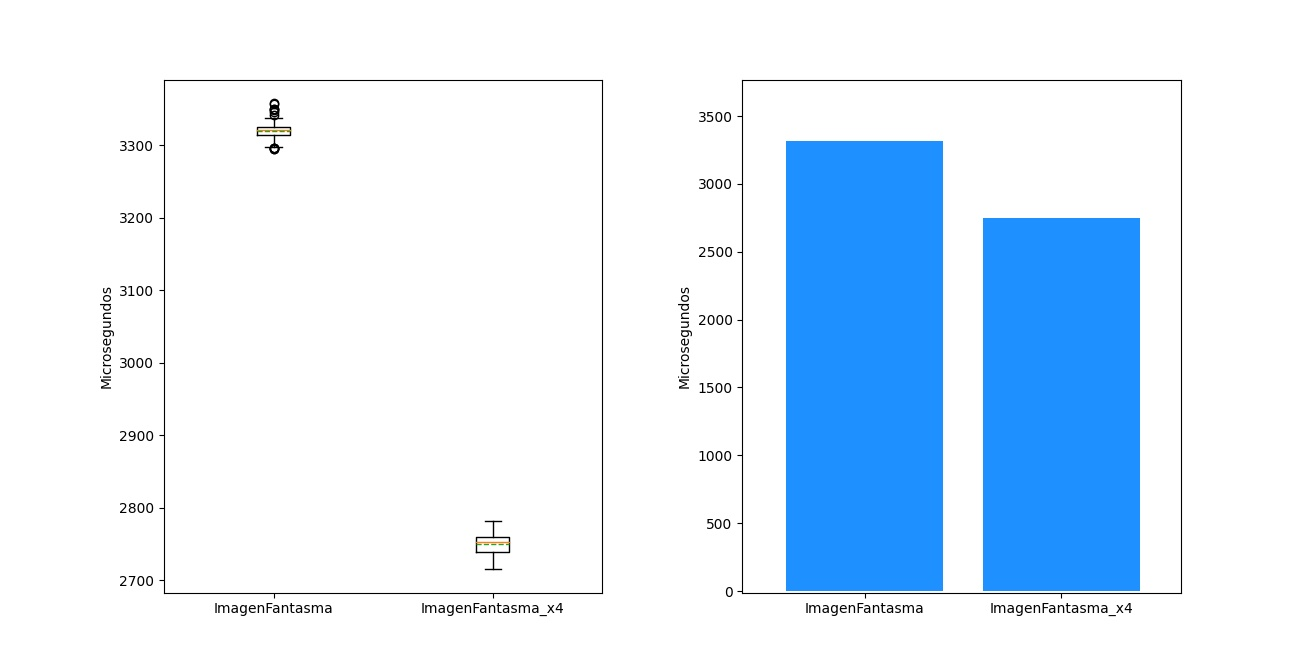
\includegraphics[scale=0.55]{img/x41.jpeg}
	\end{center}
	\caption{Dispersión y media de ejecución en microsegundos}
	\label{exp2_m}
\end{figure}
Viendo cómo se distribuyen los microsegundos para el filtro normal y el experimental, se puede apreciar una mejoría de alrededor unos 600 microsegundos teniendo en referencia los 3300 que toma el filtro original. De nuevo es difícil de apreciar por la medida de tiempo pero es significativa.

\begin{figure}[!h]
    \begin{center}
	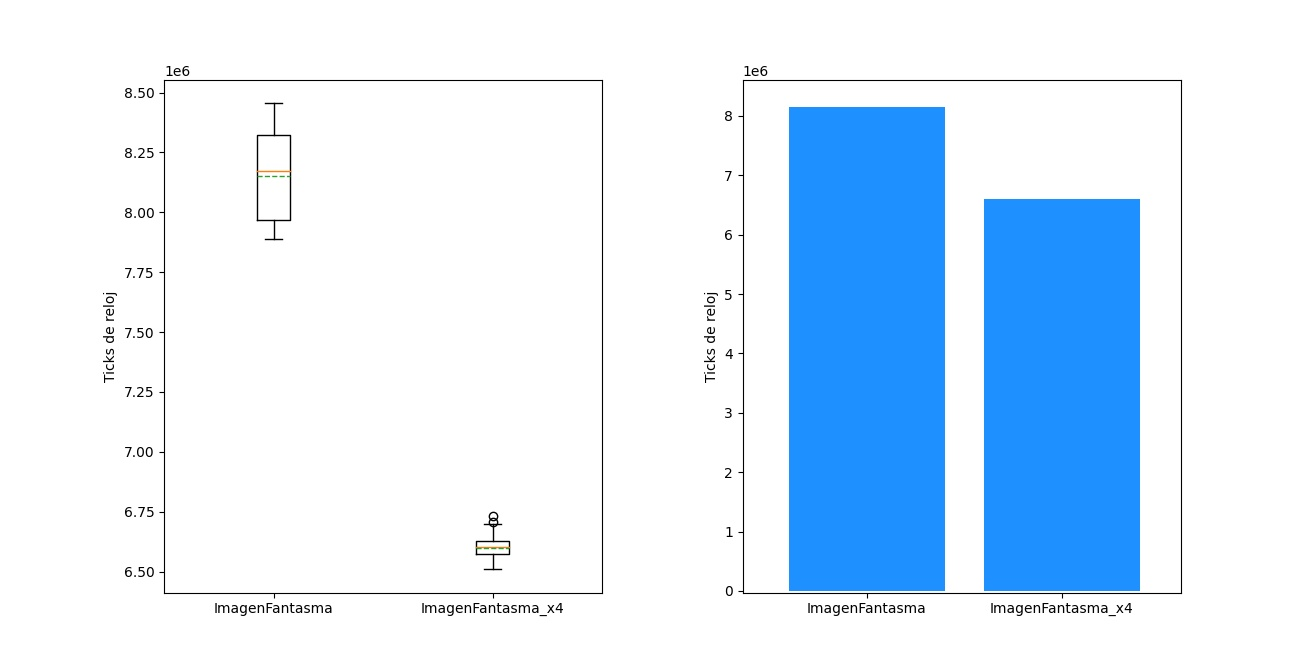
\includegraphics[scale=0.55]{img/x42.jpeg}
	\end{center}
	\caption{Dispersión y media de los ticks reloj por ejecución}
	\label{exp2_c}
\end{figure}

En cuanto a los ticks de relojs, el filtro que procesa de a 4 pixeles ronda en los 6 millones y medio de clocks, a diferencia de los 8.25 millones que toma el filtro normal.
La mejora de performance es notable.

\subsubsection{Conclusión}
 Los resultados son los esperados. La cantidad de instrucciones por ciclo es mayor, pero al realizar los cálculos relacionados a la submatriz de offsets, se reducen los accesos a memoria a la mitad, junto a los ciclos de procesar la imagen completa. Y los datos en los gráficos son la prueba de eso.
